\documentclass[fleqn, 11pt]{article}

\usepackage{verbatim}
\usepackage{amsmath}
\DeclareMathOperator*{\argmin}{arg\,min}
\DeclareMathOperator*{\argmax}{arg\,max}
\usepackage{amssymb}
\usepackage{amsthm}
\usepackage{hyperref}
\usepackage{ulem}
\usepackage{enumitem}
\usepackage[top=1.0in, left=0.75in, right=0.75in, bottom=0.75in]{geometry}
\usepackage{graphicx}

\setlength{\headheight}{15pt}

\usepackage{import}

\usepackage{setspace}

\newcommand{\bs}[1]{\boldsymbol{#1}}
\newcommand\norm[1]{\left\lVert#1\right\rVert}
\newcommand{\R}[0]{\mathbb{R}}
\newcommand{\HRule}{\rule{\linewidth}{0.5mm}} 

\usepackage{array}
\usepackage{caption}
\usepackage{floatrow}
\usepackage{multirow}
\usepackage{multicol}

\usepackage{chngcntr}
\counterwithin*{equation}{section}
\counterwithin*{equation}{subsection}

\usepackage{sectsty}
\sectionfont{\centering}

\usepackage[perpage]{footmisc}

\usepackage{fancyhdr}
\pagestyle{fancy}
\fancyhf{}
\lhead{190100036 \& 190100044}
\rhead{CS 754: Assignment 5}
\renewcommand{\footrulewidth}{1.0pt}
\cfoot{Page \thepage}

\setlength{\parindent}{0em}
\renewcommand{\arraystretch}{2}%

\title{Assignment 5: CS 754}
\author{ 
\begin{tabular}{|c|c|}
     \hline
     \textsf{Krushnakant Bhattad} & \textsf{Devansh Jain} \\
     \hline
     \textsf{190100036} & \textsf{190100044}\\
     \hline
\end{tabular}
}
\date{April 19, 2021}


\begin{document}

\maketitle
\tableofcontents
\thispagestyle{empty}
\setcounter{page}{0}

\renewcommand{\arraystretch}{1}%

\newpage
\section*{Question 1}
\addcontentsline{toc}{section}{Question 1}
\setcounter{equation}{0}

\subsection*{Part (2)}

\textbf{Question: }
In Eqn. (6), which terms are obtained from the prior and which terms are obtained from the likelihood?
What is the prior used in the paper? What is the likelihood used in the paper?

\hrulefill

\textbf{Answer: }

\subsection*{The Terms}

Let's break down the function as: 
\begin{center}
$    \begin{aligned}
\text{Expression 1: } & \displaystyle \sum_{i,k} \rho(f_{i,k} \cdot I_1) + \rho(f_{i,k} \cdot (I-I_1)) \\
\text{Expression 2: } & \lambda \displaystyle \sum_{i \in S_1,k} \rho(f_{i,k} \cdot I_1 -  f_{i,k} \cdot I )  + 
\lambda \displaystyle \sum_{i \in S_2,k} \rho(f_{i,k} \cdot I_1 ) 
\end{aligned}$
\end{center}

Then, we note that the terms in Expression 1 have come from our prior belief, 
and that the terms in expression 2 have come from the likelihood term.


\subsection*{The Prior used}

The Prior used in the paper is the sparsity prior.

\smallskip

A sparse distribution can be achieved by mixing only two laplacian
distributions: a narrow distribution centered on zero and a broad distribution centered on zero. 

\smallskip

For example, 

\begin{center}
    $\text{Pr}(x) = \dfrac{\pi_1}{2s_1}e^{-|x|/s_1} + \dfrac{\pi_2}{2s_2}e^{-|x|/s_2}     $  \\
\end{center}
    where learned values  found are $ s_1 = 0.01, s_2 = 0.05, \pi_1 = 0.4, \pi_2 = 0.6 $.

\medskip

We define a distribution over
images by assuming that derivative filters are independent over space and orientation so that our prior
over images is given by:
\begin{center}
    $\text{Pr}(I) \approx \displaystyle  \prod_{i,k} \text{Pr}(f_{i,k} \cdot I)  $
\end{center}
where  $f \cdot I$ denotes the inner product between a linear filter $f$ and an image $I$ , 
and $f_{i,k} $ is the $k^{\text{th}}$
derivative filter centered on pixel $i$ . We enforce this prior using negative log of the probability in the cost function.


\subsection*{The Likelihood used}

The likelihood used in the paper depends upon two things: first, the given input image $I$.

\smallskip

Next, the two sets of image
locations $S_1, S_2$ so that gradients in location $S_1$ belong to layer 1 and 
gradients in location $S_2$ belong to layer 2 .

\smallskip

We enforce the agreement with the labeled gradients using the terms in expression 2. 

\medskip

$\displaystyle \sum_{i \in S_1,k} \rho(f_{i,k} \cdot I_1 -  f_{i,k} \cdot I ) $ enforces that  gradients in location $S_1$ belong to layer 1,
and 

\medskip

$ \displaystyle \sum_{i \in S_2,k} \rho(f_{i,k} \cdot I_1 )   $ enforces that  gradients in location $S_2$ belong to layer 2 (here we use $I-I_2=I_1$)







\subsection*{Part (3)}

\textbf{Question: }

\smallskip

Why does the paper use a likelihood term that is different from the Gaussian prior?

\hrulefill

\smallskip

\textbf{Answer: }

\smallskip

A remarkably robust property of natural images that has received much attention lately is the fact that
when derivative filters are applied to natural images, the filter outputs tend to be sparse. The log-histograms
of derivative filters lie below the straight line connecting the minimal and maximal values. 
We refer to such distributions as sparse. 

\smallskip

For example, it has been illustrated in literature that 
the histogram of the vertical derivative filter is peaked at zero and falls
off much faster than a Gaussian.

\smallskip

The following figure shows a natural image on the left side, and on the right side, a plot of $d_y$ 
derivative filter output in blue; and a dashed straight line connecting the minimal and maximal values.
This supports what we have said so far.

\begin{center}
    \includegraphics[scale=0.5]{derivative filter.png}
\end{center}


When we look at 
the logarithm of the histogram the curve is
always below the straight line connecting the maximum and minimum values. 


\smallskip

This should be contrasted
with the Gaussian distribution (that is always above the straight line) or the Laplacian distribution (that
is simply a straight line in the log domain)

\smallskip

It was shown (in literature) that the fact that the log
distribution is always below the straight line, is crucial for obtaining transparency decomposition from
a single image.

\smallskip

Distributions that are above the straight line (like the gaussian) will prefer to split an edge of unit contrast
into two edges (one in each layer) with half the contrast, but what we want, is achieved by 
distributions below the line: They will prefer
decompositions in which the edge only appears in one of the layers but not in the other.
(that is, treat the images $I_1$, and $I_2$ as separate and not mixed unlike the gaussian distribution). 

That is why we use the sparse distribution, which was defined in the previous part in the prior section. 









\newpage
\section*{Question 2}
\addcontentsline{toc}{section}{Question 2}
\setcounter{equation}{0}

\subsection*{Instructions for running the code:}
\begin{itemize}[noitemsep]
    \item After extracting submitted file, look for a directory named \texttt{q2}, and \texttt{cd} (change directory) to it.
    \item Run the file \texttt{q2.m}.
    \item The plots can be found in \texttt{./plots/}.
\end{itemize}

\medskip

\subsection*{Deriving expression for maximum a posteriori (MAP) Estimate}
Given:
\begin{equation*}
    \begin{aligned}
        \bs{y} &= \bs{\Phi x} + \bs{\eta} \\
        \bs{y} &\in \mathbb{R}^m \\
         \bs{\Phi} &\in \mathbb{R}^{m \times n} \ (m \ll n) \\
         \bs{x} &\in \mathbb{R}^n, \bs{x} \sim \mathcal{N}(0, \bs{\Sigma})\\
         \bs{\eta} &\in \mathbb{R}^m, \bs{\eta} \sim \mathcal{N}(0,\sigma^2\bs{I}_{m \times m}) \\
    \end{aligned}
\end{equation*}

MAP of $\bs{x}$:
\begin{equation*}
    \begin{aligned}
        \bs{\hat{x}}
        % &= \argmax_{\bs{x}} p(\bs{x} \vert \bs{y}, \bs{\phi}) = \argmax_{\bs{x}} p(\bs{x} \vert \bs{y} \vert \bs{\phi}) \\
        %     &= \argmax_{\bs{x}} p(\bs{y} \vert \bs{x} \vert \bs{\phi}) \cdot p(\bs{x} \vert \bs{\phi}) \\
            &= \argmax_{\bs{x}} p(\bs{y} \vert \bs{x}, \bs{\phi}) \cdot p(\bs{x}) \\
            & (\text{Noise $\bs{\eta} = \bs{y} - \bs{\phi} \bs{x}$ is Gaussian modelled, so is the original vector $\bs{x}$}) \\
            &= \argmax_{\bs{x}} \left( \frac{1}{(\sigma^{2m})^{0.5} (2\pi)^{m/2}} \exp \left(-\frac{(\bs{y} - \bs{\phi} \bs{x})^t (\sigma^2 \bs{I})^{-1} (\bs{y} - \bs{\phi} \bs{x})}{2} \right) \right) \cdot \left( \frac{1}{(\vert\bs{\Sigma}\vert)^{0.5} (2\pi)^{n/2}} \exp \left(-\frac{(\bs{x})^t (\bs{\Sigma})^{-1} (\bs{x})}{2} \right) \right) \\
            &= \argmax_{\bs{x}} \left( \frac{1}{(\sigma^{2m})^{0.5} (\vert\bs{\Sigma}\vert)^{0.5} (2\pi)^{(m+n)/2}} \right) \cdot \exp \left(-\frac{ \Vert \bs{y} - \bs{\phi} \bs{x} \Vert_2^2}{2 \sigma^2} -\frac{(\bs{x})^t (\bs{\Sigma})^{-1} (\bs{x})}{2} \right) \\
            &= \argmax_{\bs{x}} \ \exp \left(-\frac{ \Vert \bs{y} - \bs{\phi} \bs{x} \Vert_2^2}{2 \sigma^2} -\frac{(\bs{x})^t (\bs{\Sigma})^{-1} (\bs{x})}{2} \right) \quad (\text{$\sigma$, $\Sigma$ are independent of x}) \\
            &= \argmin_{\bs{x}} \left( \frac{ \Vert \bs{y} - \bs{\phi} \bs{x} \Vert_2^2}{2 \sigma^2}  +\frac{(\bs{x})^t (\bs{\Sigma})^{-1} (\bs{x})}{2} \right) \quad (\argmax_x f(x) = \argmin_x -\log f(x)) \\
            &= \argmin_{\bs{x}} f(\bs{x}, \bs{y}, \bs{\phi}, \bs{\Sigma}, \sigma) \\
    \end{aligned}
\end{equation*}
\begin{equation*}
    \begin{aligned}
        & \frac{\partial f(\bs{x}, \bs{y}, \bs{\phi}, \bs{\Sigma}, \sigma)}{\partial \bs{x}} \bigg\vert_{\bs{x} = \bs{\hat{x}}} = \frac{2 (-\bs{\phi}^t) (\bs{y} - \bs{\phi} \bs{\hat{x}})}{2 \sigma^2} + \frac{2 \bs{\Sigma}^{-1} \bs{\hat{x}}}{2} = 0 \\
        & \frac{\bs{\phi}^t \bs{y}}{\sigma^2} - \frac{\bs{\phi}^t \bs{\phi} \bs{\hat{x}}}{\sigma^2} - \bs{\Sigma}^{-1} \bs{\hat{x}} = 0 \\
        & \frac{\bs{\phi}^t \bs{y}}{\sigma^2} = \left( \frac{\bs{\phi}^t \bs{\phi}}{\sigma^2} + \bs{\Sigma}^{-1} \right) \bs{\hat{x}} \\
        & \bs{\hat{x}} = \left( \frac{\bs{\phi}^t \bs{\phi}}{\sigma^2} + \bs{\Sigma}^{-1} \right)^{-1} \frac{\bs{\phi}^t \bs{y}}{\sigma^2} \\
    \end{aligned}
\end{equation*}
Making the calculation computationally faster:
\begin{equation*}
    \begin{aligned}
        \left( \frac{\bs{\phi}^t \bs{\phi}}{\sigma^2} + \bs{\Sigma}^{-1} \right)^{-1} &= \left( \bs{\Sigma}^{-1} + \bs{\phi}^t \left(\frac{\bs{I}_{m \times m}}{\sigma^2}\right) \bs{\phi} \right)^{-1} \\
            &= \left( \bs{\Sigma} - \bs{\Sigma} \bs{\phi}^t \left( (\sigma^2 \bs{I}_{m \times m}) + (\bs{\phi} \bs{\Sigma} \bs{\phi}^t) \right)^{-1} \bs{\phi} \bs{\Sigma} \right) \quad (\text{Using Woodbury matrix identity}) \\
    \end{aligned}
\end{equation*}
\begin{equation*}
    \begin{aligned}
        \bs{\hat{x}} &= \left( \bs{\Sigma} - \bs{\Sigma} \bs{\phi}^t \left( (\sigma^2 \bs{I}_{m \times m}) + (\bs{\phi} \bs{\Sigma} \bs{\phi}^t) \right)^{-1} \bs{\phi} \bs{\Sigma} \right) \frac{\bs{\phi}^t \bs{y}}{\sigma^2} \\
            &= \frac{\left( \bs{\Sigma\phi}^t - \bs{\Sigma\phi}^t \left( (\sigma^2 \bs{I}_{m \times m}) + (\bs{\phi\Sigma\phi}^t) \right)^{-1} \bs{\phi\Sigma\phi}^t \right) \bs{y}}{\sigma^2} \\
        \bs{\hat{x}} &= \left(\bs{C_1} - \bs{C_1} \left( \sigma^2 \bs{I}_{m \times m} + \bs{C_2} \right)^{-1} \bs{C_2} \right) \bs{y} / \sigma^2 \\
            & \quad \text{where, $\bs{C_1} = \bs{\Sigma\phi}^t$ and $\bs{C_2} = \bs{\phi\Sigma\phi}^t$}
    \end{aligned}
\end{equation*}

\medskip

\subsection*{Explaining the Code}
\subsubsection*{Generating original signal}
\begin{enumerate}
    \item Generating a random orthonormal matrix
        \begin{verbatim}
        U = zeros(n);
        vi = randn(n,1);
        U(:,1) = vi ./ norm(vi);
        for i=2:n
          nrm = 0;
          while nrm < tol
            vi = randn(n,1);
            vi = vi - U(:,1:i-1) * (U(:,1:i-1)' * vi);
            nrm = norm(vi);
          end
          U(:,i) = vi ./ nrm;
        end
        \end{verbatim}

    \item Generating Co-variance Matrix
        \begin{verbatim}
        Sigma = U * diag((1:n).^(-alpha)) * U';
        \end{verbatim}

    \item Generating 10 n-dimensional vectors
        \begin{verbatim}
        xs = mvnrnd(zeros(n,1), Sigma, 10)';
        \end{verbatim}
\end{enumerate}

\subsubsection*{Generating measured signal}
\begin{enumerate}
    \item Generating a random sensing matrix
        \begin{verbatim}
        phi = randn(m, n) / sqrt(m);
        \end{verbatim}

    \item Generating noisy measurement
        \begin{verbatim}
        y = phi * xs(:, i);
        sig = 0.01 * mean(abs(y));
        y = y + mvnrnd(zeros(m, 1), eye(m)*sig^2, 1)';
        \end{verbatim}
\end{enumerate}

\subsubsection*{Reconstruction}
\begin{enumerate}
    \item Variables used in reconstruction (for faster computation)
        \begin{verbatim}
        SpT = Sigma * phi';
        pSpT = phi * SpT;
        \end{verbatim}

    \item Reconstruction of x
        \begin{verbatim}
        x = (SpT - SpT/(eye(m)*sig^2 + pSpT)*pSpT) * y / (sig^2);
        \end{verbatim}

    \item Calculating Avg. Relative RMSE
        \begin{verbatim}
        rmse(i) = sqrt(mean((x - xs(:,i)).^2))/sqrt(mean(xs(:,i).^2));
        \end{verbatim}
\end{enumerate}

\medskip

\subsection*{Results}

\begin{figure}[H]
    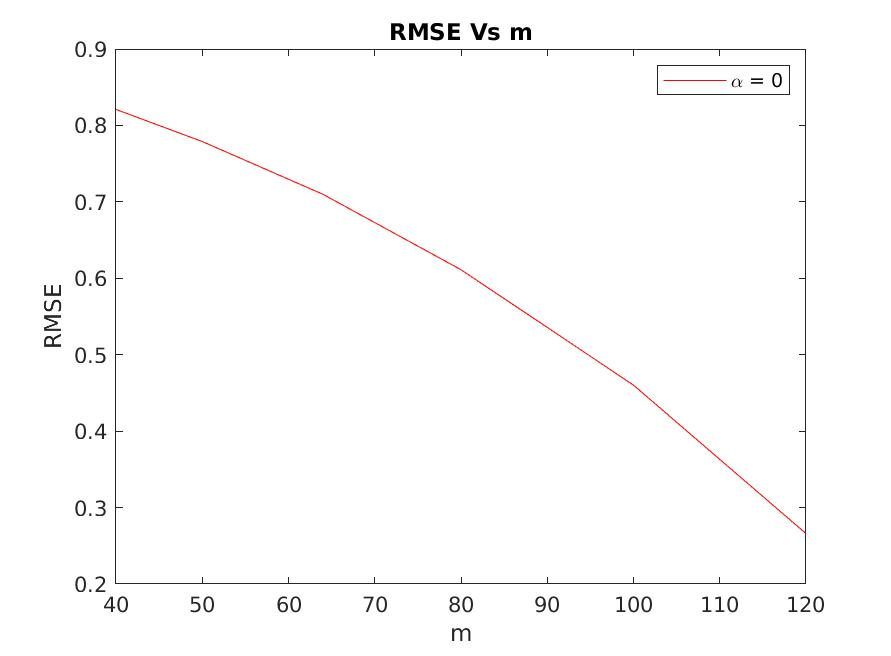
\includegraphics[scale=0.4]{0.jpg}
\end{figure}
\begin{figure}[H]
    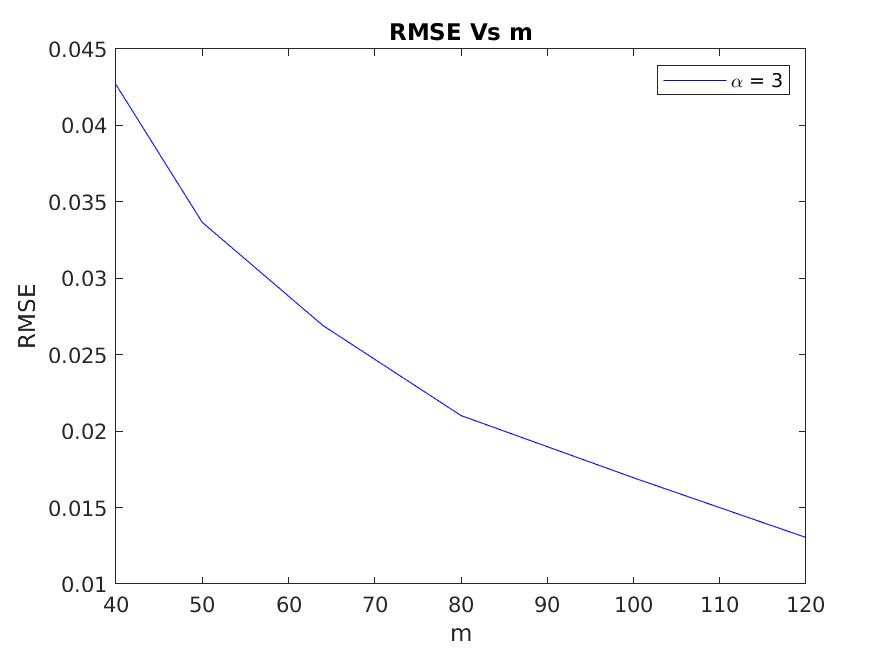
\includegraphics[scale=0.4]{3.jpg}
\end{figure}
\begin{figure}[H]
    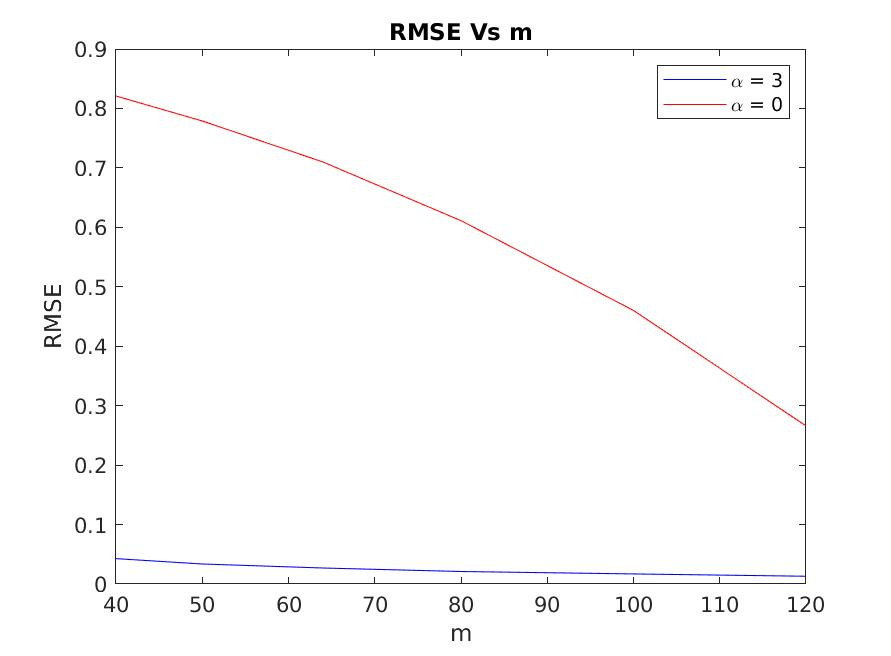
\includegraphics[scale=0.4]{both.jpg}
\end{figure}

\begin{table}[H]
    \centering
    \begin{tabular}{|c||c|c||}
        \hline
        \multirow{3}{*}{$m (< n=128 )$} & \multicolumn{2}{c||}{Avg. Relative RMSE} \\
        & \multicolumn{2}{c||}{$\left( \dfrac{1}{10} \sum\limits_{i=1}^{10} \dfrac{\Vert \bs{\hat{x_i}} - \bs{x_i} \Vert_2}{\Vert \bs{x_i} \Vert_2} \right)$}\\
        \cline{2-3}
        & $\alpha = 0$ & $\alpha = 3$ \\
        \hline
        40 & 0.820906 & 0.042668 \\
        \hline
        50 & 0.778914 & 0.033657 \\
        \hline
        64 & 0.709862 & 0.026905 \\
        \hline
        80 & 0.611197 & 0.021020 \\
        \hline
        100 & 0.460178 & 0.016950 \\
        \hline
        120 & 0.265929 & 0.013042 \\
        \hline
    \end{tabular}
\end{table}

\medskip

\subsection*{Comments}
\begin{itemize}
    \item Average Relative RMSE decreases with increase in $m$ as expected. We have more information about the original signal, so reconstruction is better.
    \item Average Relative RMSE for $\alpha = 3$ lies in range 0.01-0.05. As the eigenvalues decay very fast (cubic speed), so several elements are zero (or almost zero) with high probability. This means that the signal $\bs{x}$ is sparse, thus giving better reconstruction.
    \item Average Relative RMSE for $\alpha = 0$ lies in range 0.25-0.85. As the eigenvalues doesn't decay, so all elements are non-zero with high probability. This means that the signal $\bs{x}$ is not sparse, thus giving poorer reconstruction.
    \item Average Relative RMSE for any $m$ is higher for smaller $\alpha$ (decay factor)
\end{itemize}


\newpage
\section*{Question 3}
\addcontentsline{toc}{section}{Question 3}
\setcounter{equation}{0}

\subsection*{Q1.}
Since $X^\star$ is the optimal solution of $\argmin_X \Vert X \Vert_\star$ s.t. $\mathcal{A}(X) = b$ (Eq 3.1) and $\mathcal{A}(X_0) = b$,
\begin{equation*}
    \begin{aligned}
        \Vert X^\star \Vert_\star \le \Vert X_0 \Vert_\star
    \end{aligned}
\end{equation*}

\subsection*{Q2.}
By construction, $X_0$ and $R_c$ have same dimension. \\
From Lemma 3.4, we have $X_0 R_c' = 0$ and $X_0' R_c = 0$. \\
Thus, $X_0$ and $R_c$ satisfy the hypothesis for Lemma 2.3. \\
So, we have
\begin{equation*}
    \begin{aligned}
        \Vert X_0 + R_c \Vert_\star = \Vert X_0 \Vert_\star + \Vert R_c \Vert_\star \implies \Vert X_0 + R_c \Vert_\star - \Vert R_0 \Vert_\star = \Vert X_0 \Vert_\star + \Vert R_c \Vert_\star - \Vert R_0 \Vert_\star
    \end{aligned}
\end{equation*}

\subsection*{Q3.}
As we have obtained $\sigma$ by singular value decomposition of $R_c$, \\
$\sigma_i$'s are the singular values of $R_c$ with $\sigma_i \ge \sigma_j \ \forall \ 1 \le i \le j \le rank(R_c)$. \\
\begin{equation*}
    \begin{aligned}
        & \sigma_j \ge \sigma_k \quad \forall j \in I_i = \{ 3r(i-1)+1, \dots, 3ri\},\ \forall k \in I_{i+1} = \{ 3ri+1, \dots, 3r(i+1)\} \\
        & \sum_{j \in I_i} \sigma_j \ge 3r \sigma_k \implies \sigma_k \le \frac{1}{3r} \sum_{j \in I_i} \sigma_j \quad \forall k \in I_{i+1}
    \end{aligned}
\end{equation*}

\subsection*{Q4.}
\begin{equation*}
    \begin{aligned}
        & \Vert R_{i+1} \Vert_F^2 = \sum_{j \in I_{i+1}} \sigma_j^2 \quad (\text{From definition of Frobenius norm on Page 6 of the paper}) \\
        & \Vert R_i \Vert_\star = \sum_{j \in I_i} \sigma_j \quad (\text{From definition of Nuclear norm on Page 6 of the paper}) \\
        & \sigma_k \le \frac{1}{3r} \sum_{j \in I_i} \sigma_j \ \forall \ k \in I_{i+1} \quad (\text{From Eq 3.5, also Q3}) \\
        & \Vert R_{i+1} \Vert_F^2 = \sum_{j \in I_{i+1}} \sigma_j^2 \le \sum_{j \in I_{i+1}} \frac{1}{9r^2} \left( \sum_{k \in I_i} \sigma_k \right)^2 = \frac{1}{3r} \left( \sum_{k \in I_i} \sigma_k \right)^2 = \frac{1}{3r} \Vert R_i \Vert_\star^2
    \end{aligned}
\end{equation*}

\subsection*{Q5.}
\begin{equation*}
    \begin{aligned}
        & \Vert R_{i+1} \Vert_F = \frac{1}{\sqrt{3r}} \Vert R_i \Vert_\star \quad (\text{Starting from Q4}) \\
        & \text{We add the equations for $i \in \{1, 2, \dots\}$ to get} \\
        & \sum_{j_{max} \ge j \ge 2} \Vert R_j \Vert_F \le \sum_{j_{max} - 1 \ge j \ge 1} \frac{1}{\sqrt{3r}} \Vert R_j \Vert_\star \le \sum_{j_{max} \ge j \ge 1} \frac{1}{\sqrt{3r}} \Vert R_j \Vert_\star
    \end{aligned}
\end{equation*}
(Singular values are non-negative, so is their sum - Nuclear norm)

\subsection*{Q6.}
\begin{equation*}
    \begin{aligned}
        & \Vert R_0 \Vert_\star \ge \Vert R_c \Vert_\star \quad (\text{From Eq 3.4}) \\
        & \frac{1}{\sqrt{3r}} \Vert R_c \Vert_\star \le \frac{1}{\sqrt{3r}} \Vert R_0 \Vert_\star
    \end{aligned}
\end{equation*}

\subsection*{Q7.}
\begin{equation*}
    \begin{aligned}
        \Vert R_0 \Vert_\star &\le \sqrt{rank(R_0)} \Vert R_0 \Vert_F \quad (\text{From Eq 2.1 on Page 6 of the paper}) \\
            &\le \sqrt{2rank(X_0)} \Vert R_0 \Vert_F = \sqrt{2r} \Vert R_0 \Vert_F \quad (\text{Lemma 3.4}) \\ \\
            & \frac{1}{\sqrt{3r}} \Vert R_0 \Vert_\star \le \frac{\sqrt{2r}}{\sqrt{3r}} \Vert R_0 \Vert_F
    \end{aligned}
\end{equation*}

\subsection*{Q8.}
As mentioned on Page 9 of the paper, ``For matrices, the rank function is subadditive." \\
$\Vert R_0 + R_1 \Vert_\star \le \Vert R_0 \Vert_\star + \Vert R_1 \Vert_\star$. \\
From Lemma 3.4, $\Vert R_0 \Vert_\star \le 2r$. \\
From construction of $R_1$, $\Vert R_1 \Vert_\star \le 3r$. \\
So, $\Vert R_0 + R_1 \Vert_\star \le 5r$, i.e., rank of $R_0 + R_1$ is at most $5r$.

\subsection*{Q9.}
\begin{equation*}
    \begin{aligned}
        \Vert \mathcal{A}(R) \Vert &= \Vert \mathcal{A}(R_0 + R_1 + \sum_{j \ge 2} R_j) \Vert \quad (\text{By construction of $R_0$ and $R_c$}) \\
            &= \Vert \mathcal{A}\left(R_0 + R_1\right) + \sum_{j \ge 2} \mathcal{A}(R_j) \Vert \quad (\text{$\mathcal{A}$ is a linear map}) \\
            &\ge \Vert \mathcal{A}\left(R_0 + R_1\right) \Vert - \Vert \sum_{j \ge 2} \mathcal{A}(R_j) \Vert \quad (\text{Triangle inequality}) \\
            &\ge \Vert \mathcal{A}\left(R_0 + R_1\right) \Vert - \sum_{j \ge 2} \Vert \mathcal{A}(R_j) \Vert \quad (\text{Triangle inequality})
    \end{aligned}
\end{equation*}

\subsection*{Q10.}
Using the definition of restricted isometry constant (Eq 3.2),
\begin{equation*}
    \begin{aligned}
        & (1 - \delta_{5r}) \Vert R_0 + R_1 \Vert_F \le \Vert \mathcal{A}(R_0 + R_1) \Vert \le (1 + \delta_{5r}) \Vert R_0 + R_1 \Vert_F \quad (\text{From Q8, $R_0 + R_1$ has rank at most $5r$}) \\
        & (1 - \delta_{3r}) \Vert R_i \Vert_F \le \Vert \mathcal{A}(R_i) \Vert \le (1 + \delta_{3r}) \Vert R_i \Vert_F  \ \forall i \ge 2 \quad (\text{By construction, $R_i$s have rank at most $3r$})
    \end{aligned}
\end{equation*}
\begin{equation*}
    \begin{aligned}
        \Vert \mathcal{A}(R) \Vert &\ge\Vert \mathcal{A}\left(R_0 + R_1\right) \Vert - \sum_{j \ge 2} \Vert \mathcal{A}(R_j) \Vert \quad (\text{Starting from Q9}) \\
            &\ge (1 - \delta_{5r}) \Vert R_0 + R_1 \Vert_F - \sum_{j \ge 2} (1 + \delta_{3r}) \Vert R_i \Vert_F \\
            &\ge (1 - \delta_{5r}) \Vert R_0 + R_1 \Vert_F - (1 + \delta_{3r}) \sum_{j \ge 2} \Vert R_i \Vert_F \\
    \end{aligned}
\end{equation*}

\subsection*{Q11.}
The assumption is that $X^\star$ is the optimal solution of $\argmin_X \Vert X \Vert_\star$ s.t. $\mathcal{A}(X) = b$ where, $b := \mathcal{A}(X_0)$.
\begin{equation*}
    \begin{aligned}
        \mathcal{A}(R) &= \mathcal{A}(X^\star - X_0) \quad (\text{By definition of R}) \\
            &= \mathcal{A}(X^\star) - \mathcal{A}(X_0) \quad (\text{$\mathcal{A}$ is a linear map}) \\
            &= b - b = 0
    \end{aligned}
\end{equation*}

\subsection*{Q12.}
\begin{equation*}
    \begin{aligned}
        & \left( (1 - \delta_{5r}) - \frac{9}{11}(1 + \delta_{3r}) \right) \Vert R_0 \Vert_F > 0 \\
        & \left( (1 - \delta_{5r}) - \frac{9}{11}(1 + \delta_{3r}) \right) > 0 \quad (\text{Frobenius norm is non-negative}) \\
        & (11 - 11\delta_{5r} - 9 - 9\delta_{3r}) > 0 \\
        & (2 - 11\delta_{5r} - 9\delta_{3r}) > 0 \\
        & 2 > 11\delta_{5r} + 9\delta_{3r} \\
    \end{aligned}
\end{equation*}


\newpage
\section*{Question 4}
\addcontentsline{toc}{section}{Question 4}
\setcounter{equation}{0}

\subsection*{Part (1)}

\textbf{Question: }

\smallskip

Why do the theorems on low rank matrix completion require that the
singular vectors be incoherent with the canonical basis (i.e. columns of the identity matrix)?

\hrulefill

\medskip

\textbf{Answer: }

\subsection*{Need}
    
To recover a low-rank matrix,
this matrix cannot be in the null space of the sampling operator giving the values of a subset of the
entries.

\smallskip

It is easy to see that if the singular vectors of a matrix $\bs{M}$ are highly concentrated,
then $\bs{M}$ could very well be in the null-space of the sampling operator.

\smallskip

For example, consider a matrix with all entries zero, except the top right entry, which is set to 1.

One would basically need to see all the entries of M to be able to recover this
matrix exactly by any method whatsoever. There is an endless list of examples of this sort.

\smallskip

Hence,
we arrive at the notion that, somehow, the singular vectors need to be sufficiently \textit{spread out}.

\smallskip

This motivates the following definition.
    
\subsection*{Coherence }

The coherence of subspace $\bs{U}$ of  $\mathbb{R}^n$ of
dimension $r$ ($\bs{U}$ has size
$n \times r$) with respect to the canonical
basis $e_i$ is defined as follows:
\begin{center}
    $\mu(\bs{U})=\dfrac{n}{r} \max_{1 \leq i \leq n} \norm{P_{\bs{U}} e_i}^2$
\end{center}

Here $P_{\bs{U}}$  is the orthogonal projection onto $\bs{U}$, 
that is $P_{\bs{U}}=\bs{U} (\bs{U}^T\bs{U})^{-1} \bs{U}^T $


\subsection*{The Condition}

We need the singular vectors to be uncorrelated with the standard basis—in order to minimize the number of observations needed to
recover a low-rank matrix.

\smallskip

Both the left and right singular vectors need to be uncorrelated with the standard basis.

\smallskip

Matrices whose column and row spaces have
low coherence cannot really be in the null space of the sampling operator.

\smallskip

Suppose the sampling matrix $\bs{M}$ has its singular value decomposition as $\bs{U}\bs{\Sigma}\bs{V}^T$

Then, we require a bound on the coherence of both matrices $\bs{U}$ and $\bs{V}$ to be bounded by some constant.

\bigskip 

That is, there should exist a positive number $\mu_0$ such that 
\begin{center}
    $\max\{ \mu(\bs{U}) , \mu(\bs{V}) \} \leq \mu_0$
\end{center}

\newpage


\subsection*{Part (2)}

\textbf{Question: }

\smallskip

How would
this coherence condition change if the sampling operator 
were changed to the one in the equation $1.13$ of the paper?

\hrulefill

\medskip

\textbf{Answer: }

\subsection*{The Sampling Operator}

We have two orthonormal bases $\bs{f_1 , \ldots , f_n}$ and $\bs{g_1 , \ldots , g_n}$
 of $\mathbb{R}^n$ , and  we are interested in solving the following: rank minimization problem 
 \begin{align*}
     \text{minimize  \hspace{10pt}  } &rank(\bs{X}) \\
     \text{subject to \hspace{10pt} }  & \bs{f_i^* X g_j} = \bs{f_i^* M g_j} \hspace{10pt} \forall \hspace{3pt} (i,j) \in \Omega
 \end{align*}
 
\subsection*{The Condition}

Now that we have re-defined our sampling operator, we now no longer need our sampled
matrix to be incoherent with the canonical basis. 

\smallskip

Now, we need our rows and columns to have incoherence 
with respect to these new bases.

\smallskip

We can express this condition as follows:

\smallskip

Firstly, we note that there exist orthonormal(unitary for complex matrices) 
transformations $\bs{F}$ and $\bs{G}$ such that for all $i = 1,2,\ldots n$, we get 
$\bs{e}_i = \bs{Ff}_i$ and also $\bs{e}_i = \bs{Gg}_i$.

\smallskip

Then, we can write:
\begin{center}
    $\bs{f_i^* X g_j} =  \bs{  e_i^*  (F X G^*) e_j    }  $
\end{center}

Hence, we need the conditions of theorems to hold for this matrix $\bs{F X G^*}$ now. 


\medskip

In other words, all that is needed is that the
column and row spaces of $\bs{M}$  
be respectively 
incoherent with the basis $(\bs{f}_i)$ and $(\bs{g}_i)$ . 



\newpage
\section*{Question 5}
\addcontentsline{toc}{section}{Question 5}
\setcounter{equation}{0}

\subsection*{Answer: }

\subsubsection*{Details of the Paper}

Title of the Paper: Finding correspondence from multiple images via sparse and low-rank decomposition

A link to the paper: \url{https://link.springer.com/content/pdf/10.1007/978-3-642-33715-4_24.pdf}

Authors: Zinan Zeng, Tsung-Han Chan, Kui Jia, Dong Xu

Publisher: Springer, Berlin, Heidelberg

Conference: European Conference on Computer Vision

Publication date: 2012/10/7

\subsection*{The problem being solved in the paper}

The correspondence problem refers to the task of finding a set of points 
in one image which can be identified as the same points in another image. 
To do this, points or features in one image are matched with the 
corresponding points or features in another image. 

\smallskip

The problem of finding the correspondence from multiple images, is a challenging combinatorial problem, and
it is the one being discussed in this paper.

\smallskip

Finding visual pattern correspondence across images or video sequences is a
long-standing problem in computer vision. It facilitates a wide range of vision
applications such as object recognition, 3D reconstruction and image
matching.

\smallskip

Here, we focus on the problem to find the feature correspondence across video sequence. 

\smallskip

Finding the global correspondence for features/patches (referred to as pat-
terns) from multiple images can be formulated as a combinatorial NP-hard problem, 
in which a set of partial permutation matrices need to be found. Meanwhile,
if each pattern is exactly the same across images, the matrix formed by the well
corresponded patterns will be low rank. 

\smallskip

For low rank representation we can incorporate
the sparse error term into the frameworks to cope with corruption and occlusion 
that inevitably exist in images and videos.

\smallskip

\subsection*{Problem Statement}


\textbf{Partial Permutation Matrices: } The set $\mathcal{P}_n$ of partial permutation matrices can be defined as follows:

\begin{center}
    $\mathcal{P}_n  = \{ \bs{P}_n \;\;\; \mid \bs{P}_n \in \{0,1\}^{K_n \times K}, 
    \;\;\; \bs{1}^T_{K_n}\bs{P_n} =   \bs{1}^T_{K}, \;\;\;     \bs{P}_n \bs{1}_K \leq  \bs{1}_{K_n}   \} $
\end{center}
where: $ \{0,1\}^{K_n \times K}$ denotes a $K_n \times K$ matrix whose elements are either 0 or 1 
and $\bs{1}_c$ denotes a column vector of all $1$ of length $c$.

\medskip

Suppose we are given N images. For each image $I_n$ we extract $K_n$ features of size $d$, 

$\bs{f}_{n,1} , \ldots , \bs{f}_{n,K} \in \mathbb{R}^d$ at $K_n$ landmark locations, 
and stack them as a matrix $\bs{F_n} =  [ \bs{f}_{n,1}  \cdots \bs{f}_{n,K_n} ] \in  \mathbb{R}^{d \times K_n} $


Our interest is to find $K$ 
intrinsic patterns for each image such that for all $n$, $K \leq K_n$, and their
correspondence among N images (i.e., N sets of K features). 

There
exist partial permutation matrices $\bs{P}_i$ such that the reordered patterns
are well corresponded.

\smallskip

That is, 
The matrix $A = [vec(\bs{F_1 P_1} )| · · · |vec(\bs{F_N P_N} )] \in  \mathbb{R}^{dK \times N} $  should be approximately low-rank.


\medskip

Moreover, in practice, error such as corruption and occlusion is common in images and
videos, thus the low rank property of the aligned matrix is likely to be violated.
To improve the robustness, such error is modeled as a sparse matrix as it only
affects a small fraction of the data.


\smallskip




\end{document}

